\section{Проектирование системы, разработка языка и алгоритма}

\subsection{Архитектура системы}

\begin{figure}
  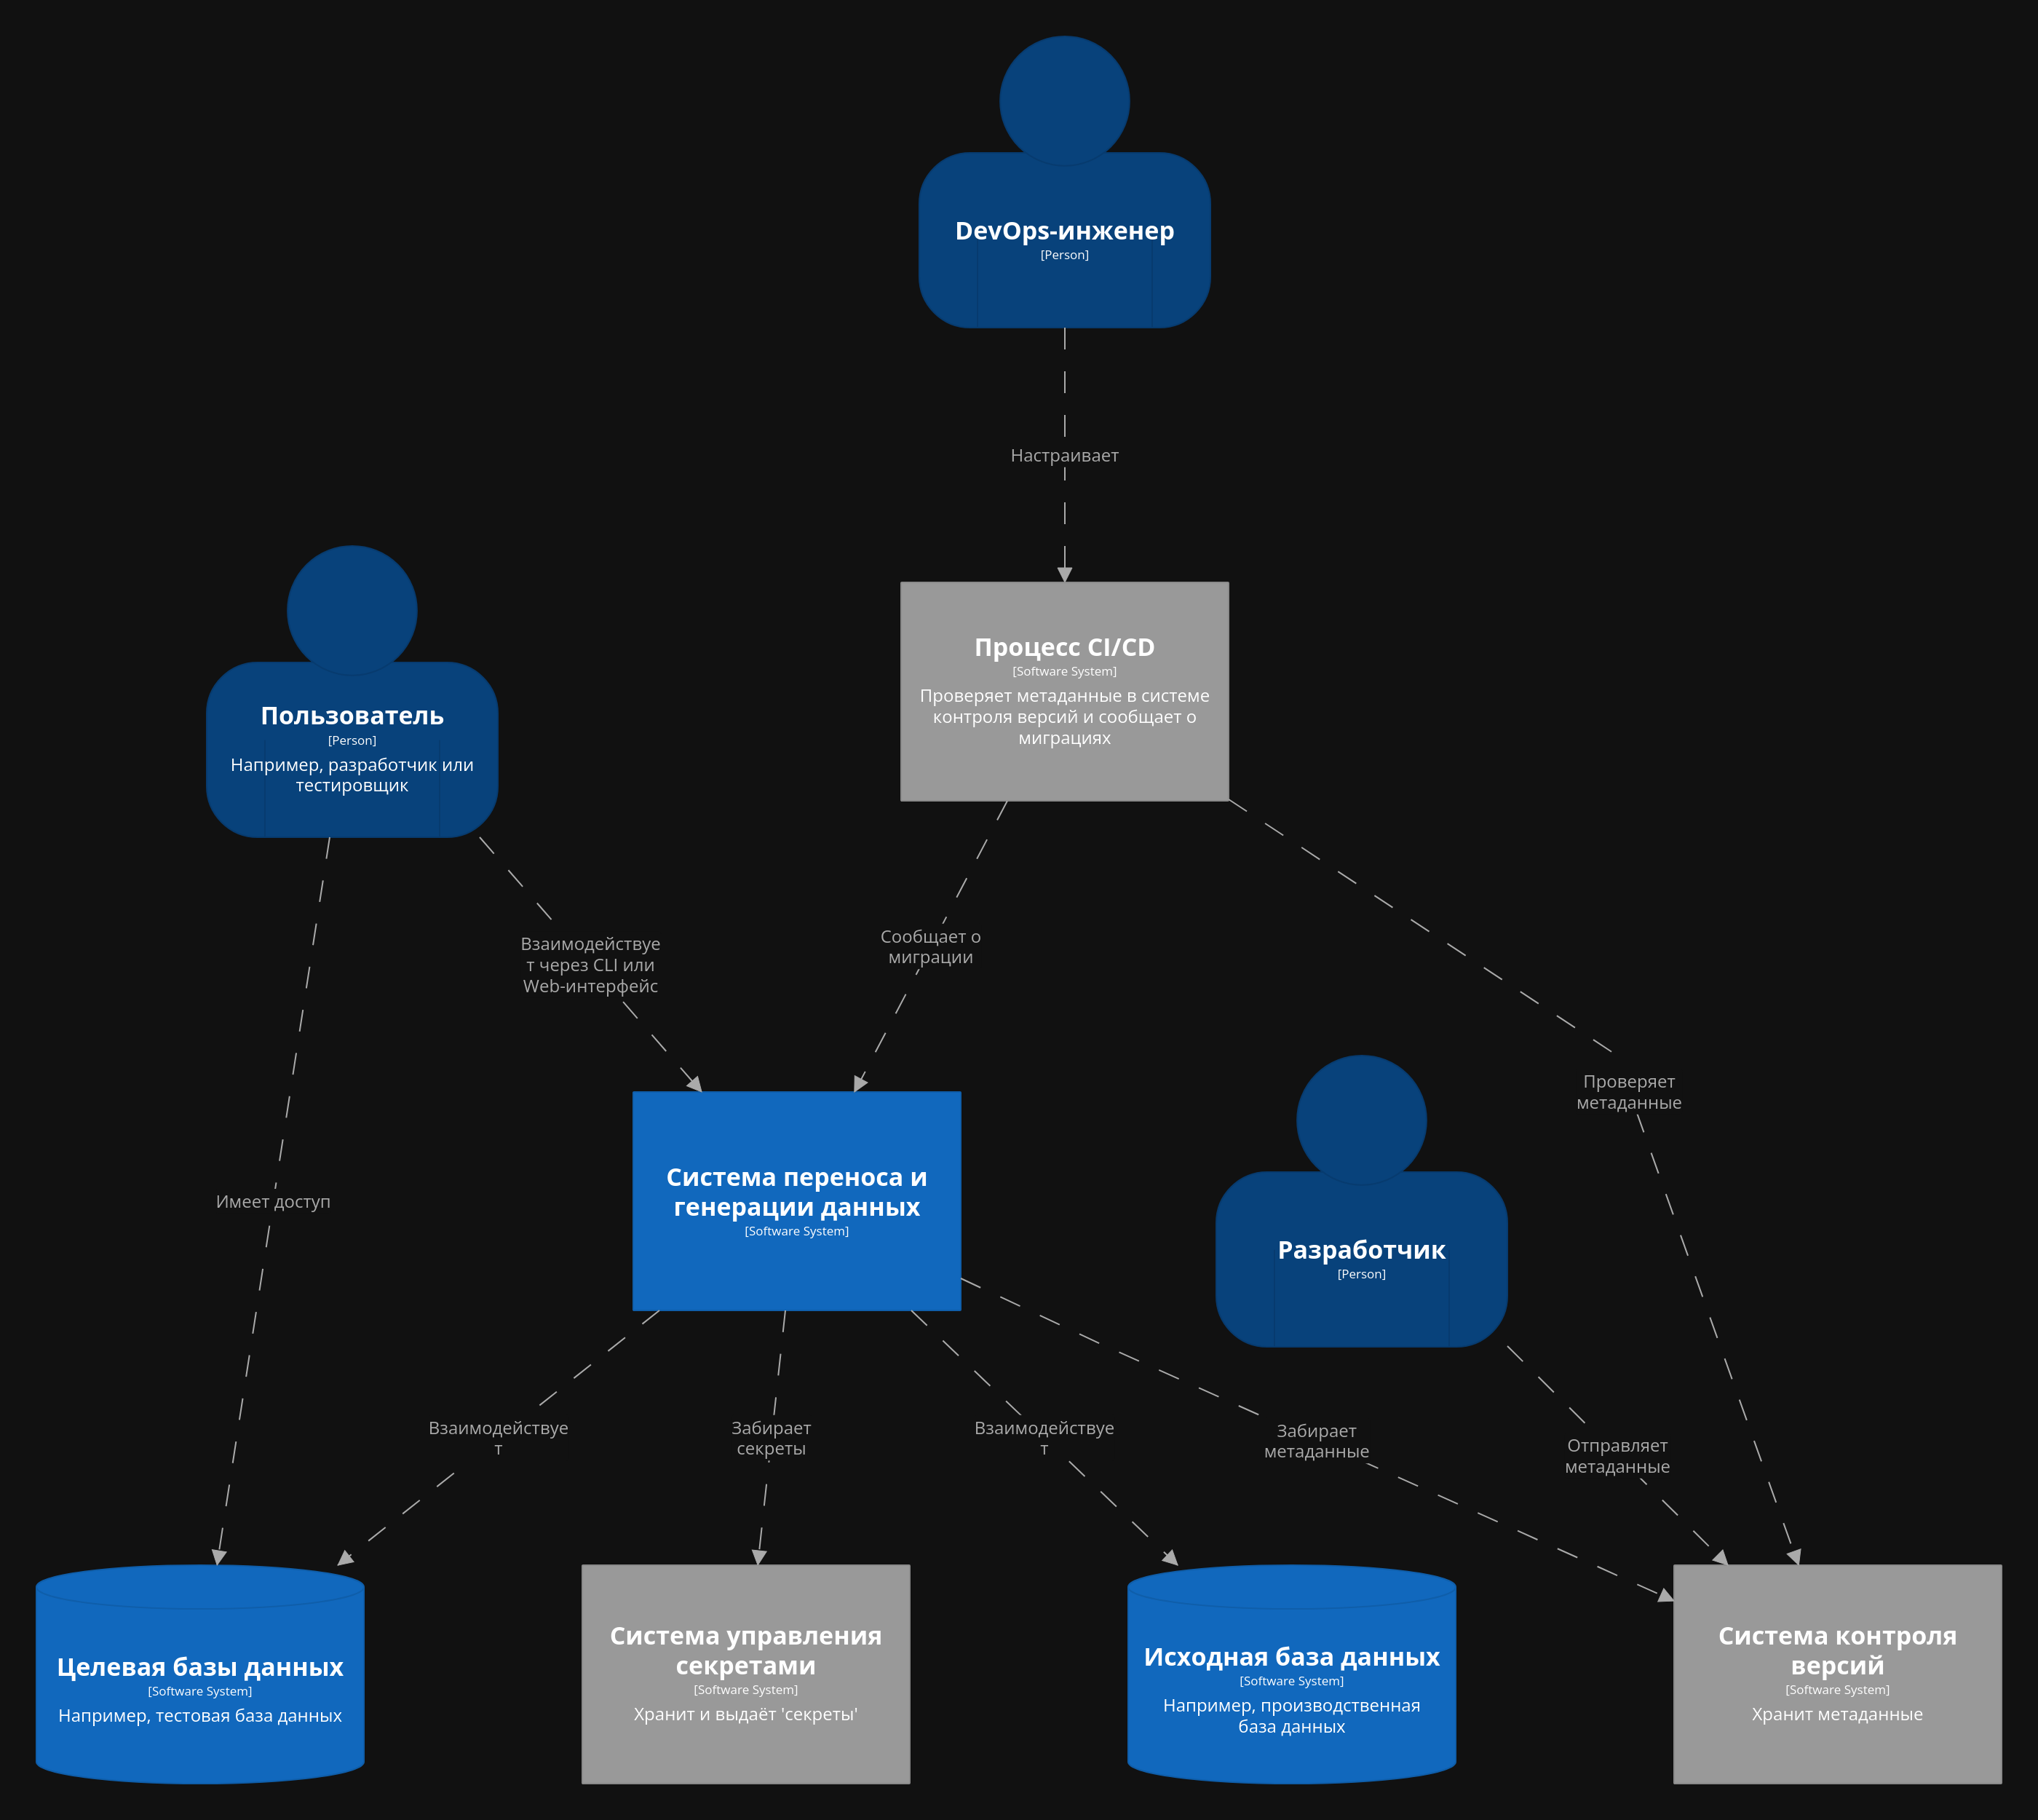
\includegraphics[scale=0.15]{./img/structurizr-SystemLandscape.png}
  \caption{System Context}
  \label{system-context}
\end{figure}

\begin{figure}
  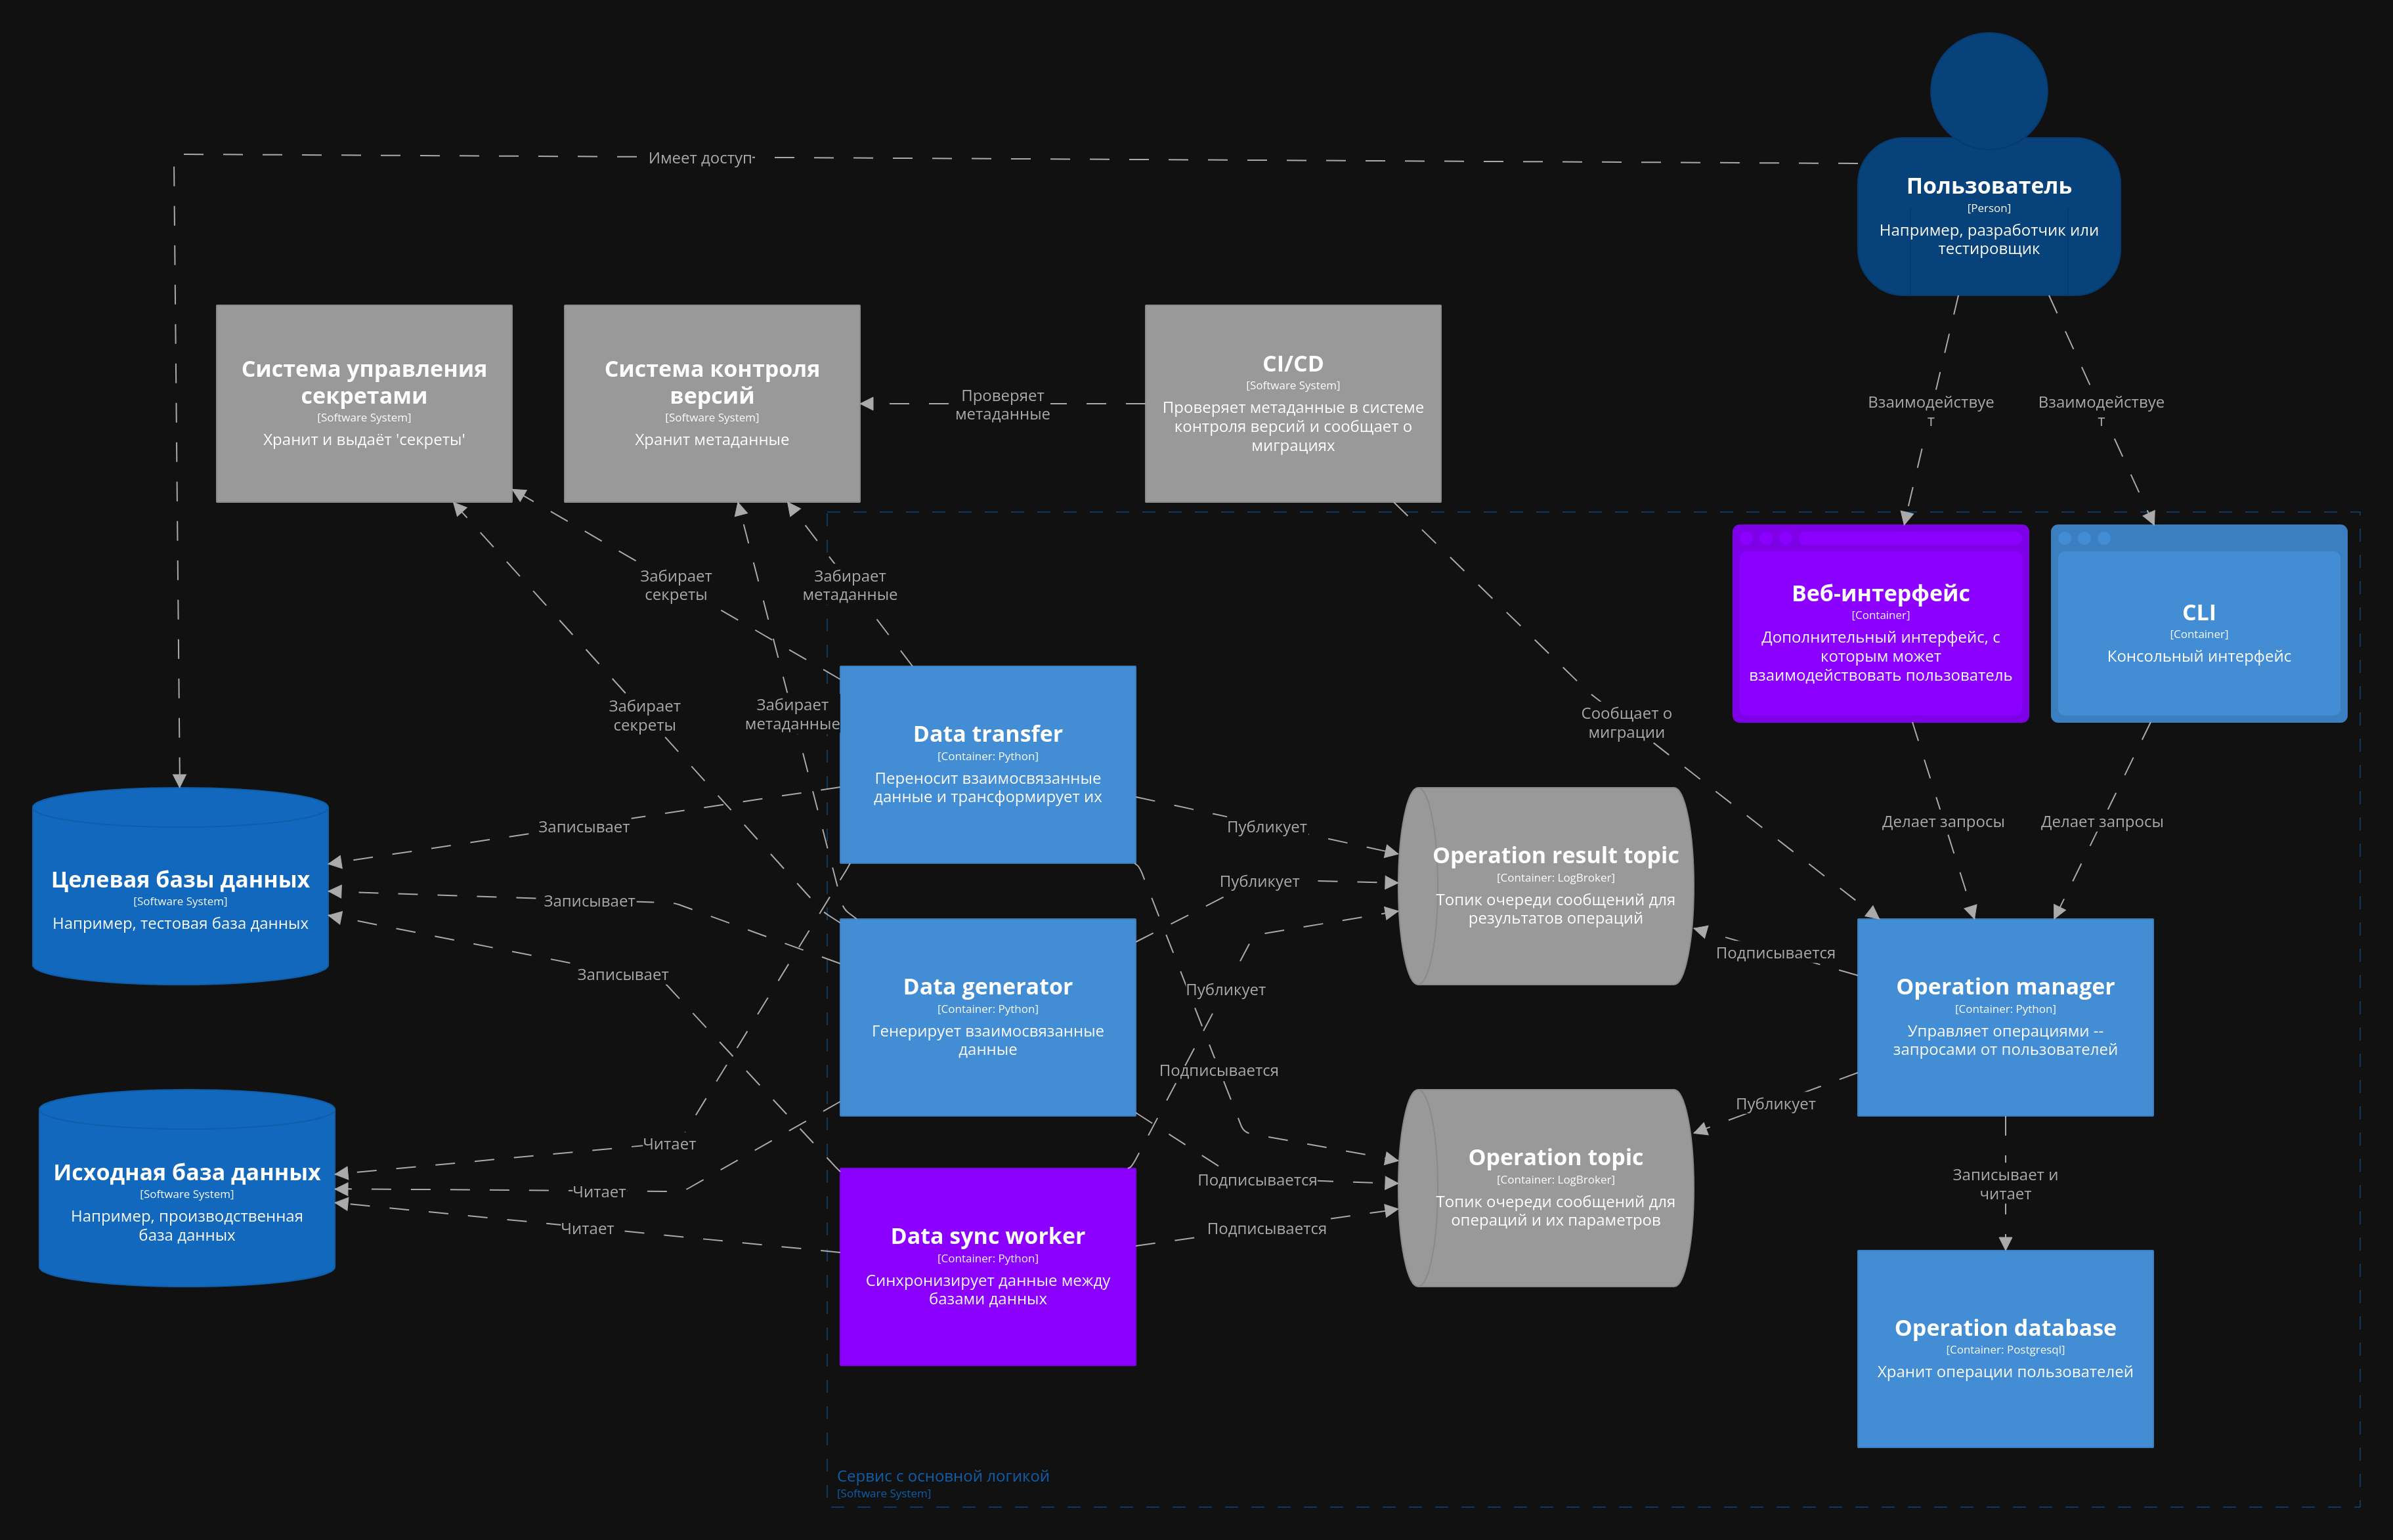
\includegraphics[scale=0.12]{./img/structurizr-Containers.png}
  \caption{Containers}
  \label{containers}
\end{figure}

\begin{figure}
  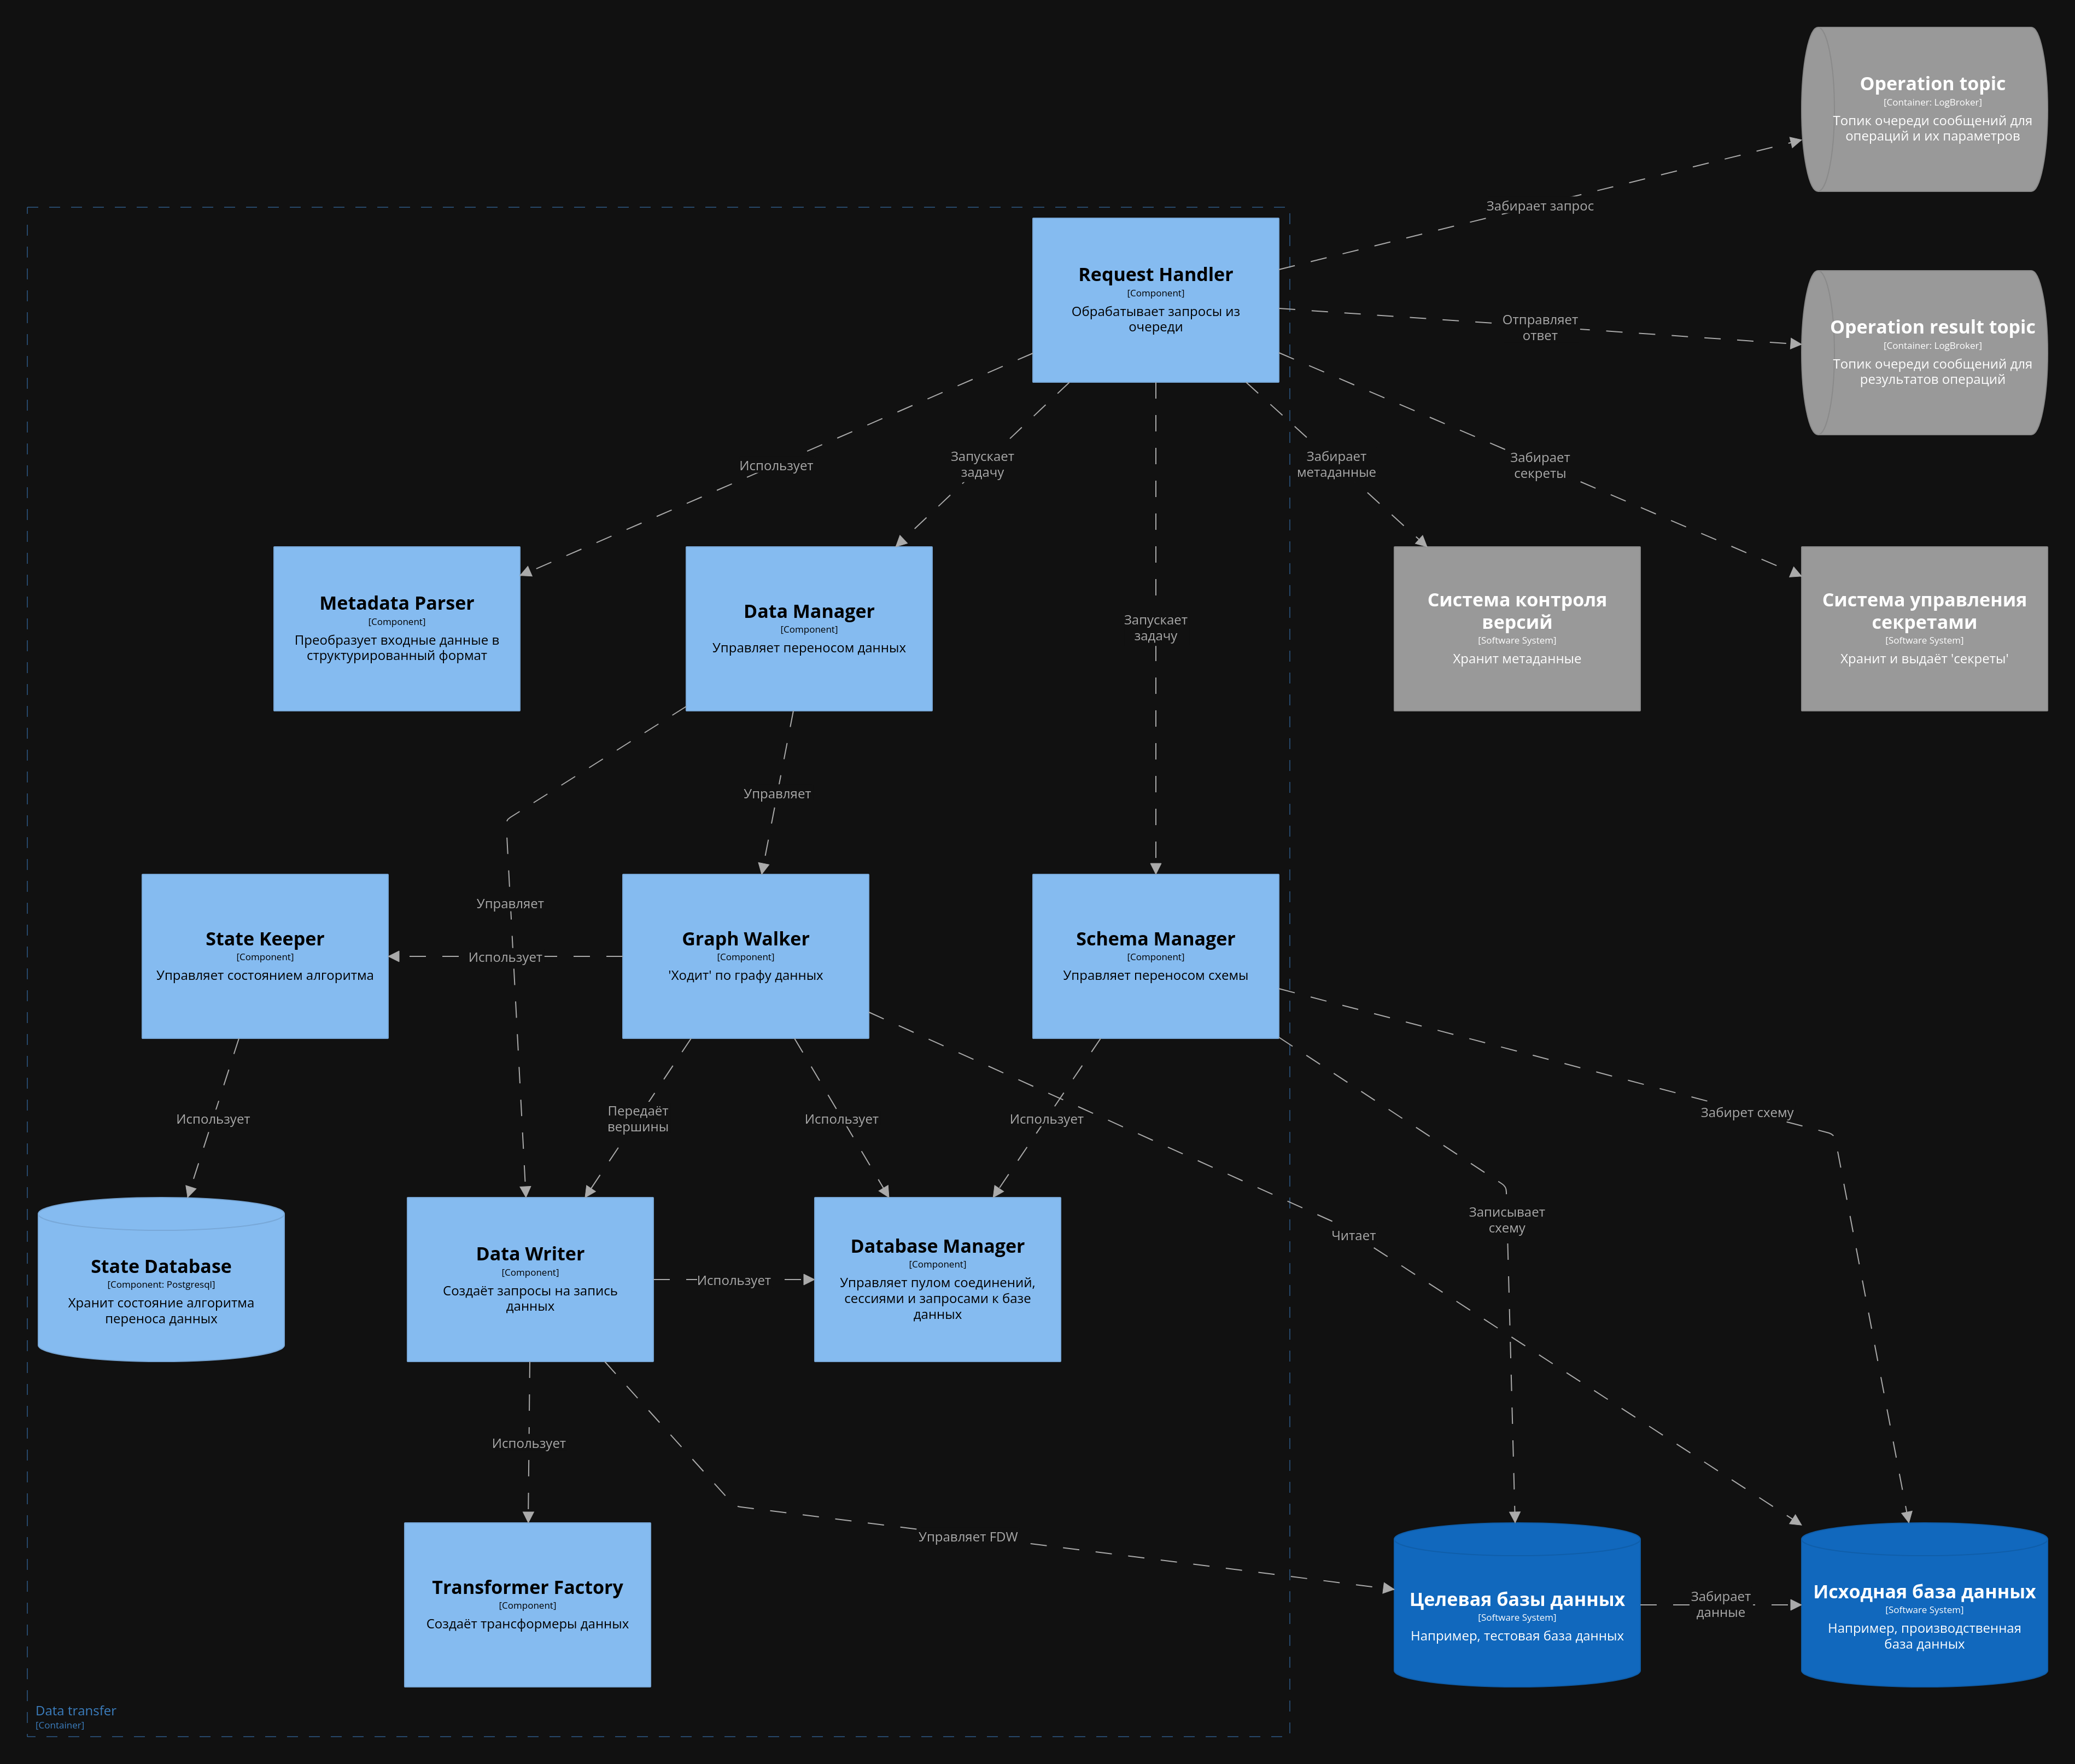
\includegraphics[scale=0.15]{./img/structurizr-DataTransferComponents.png}
  \caption{Data Transfer Components}
  \label{data-transfer-components}
\end{figure}

\begin{figure}
  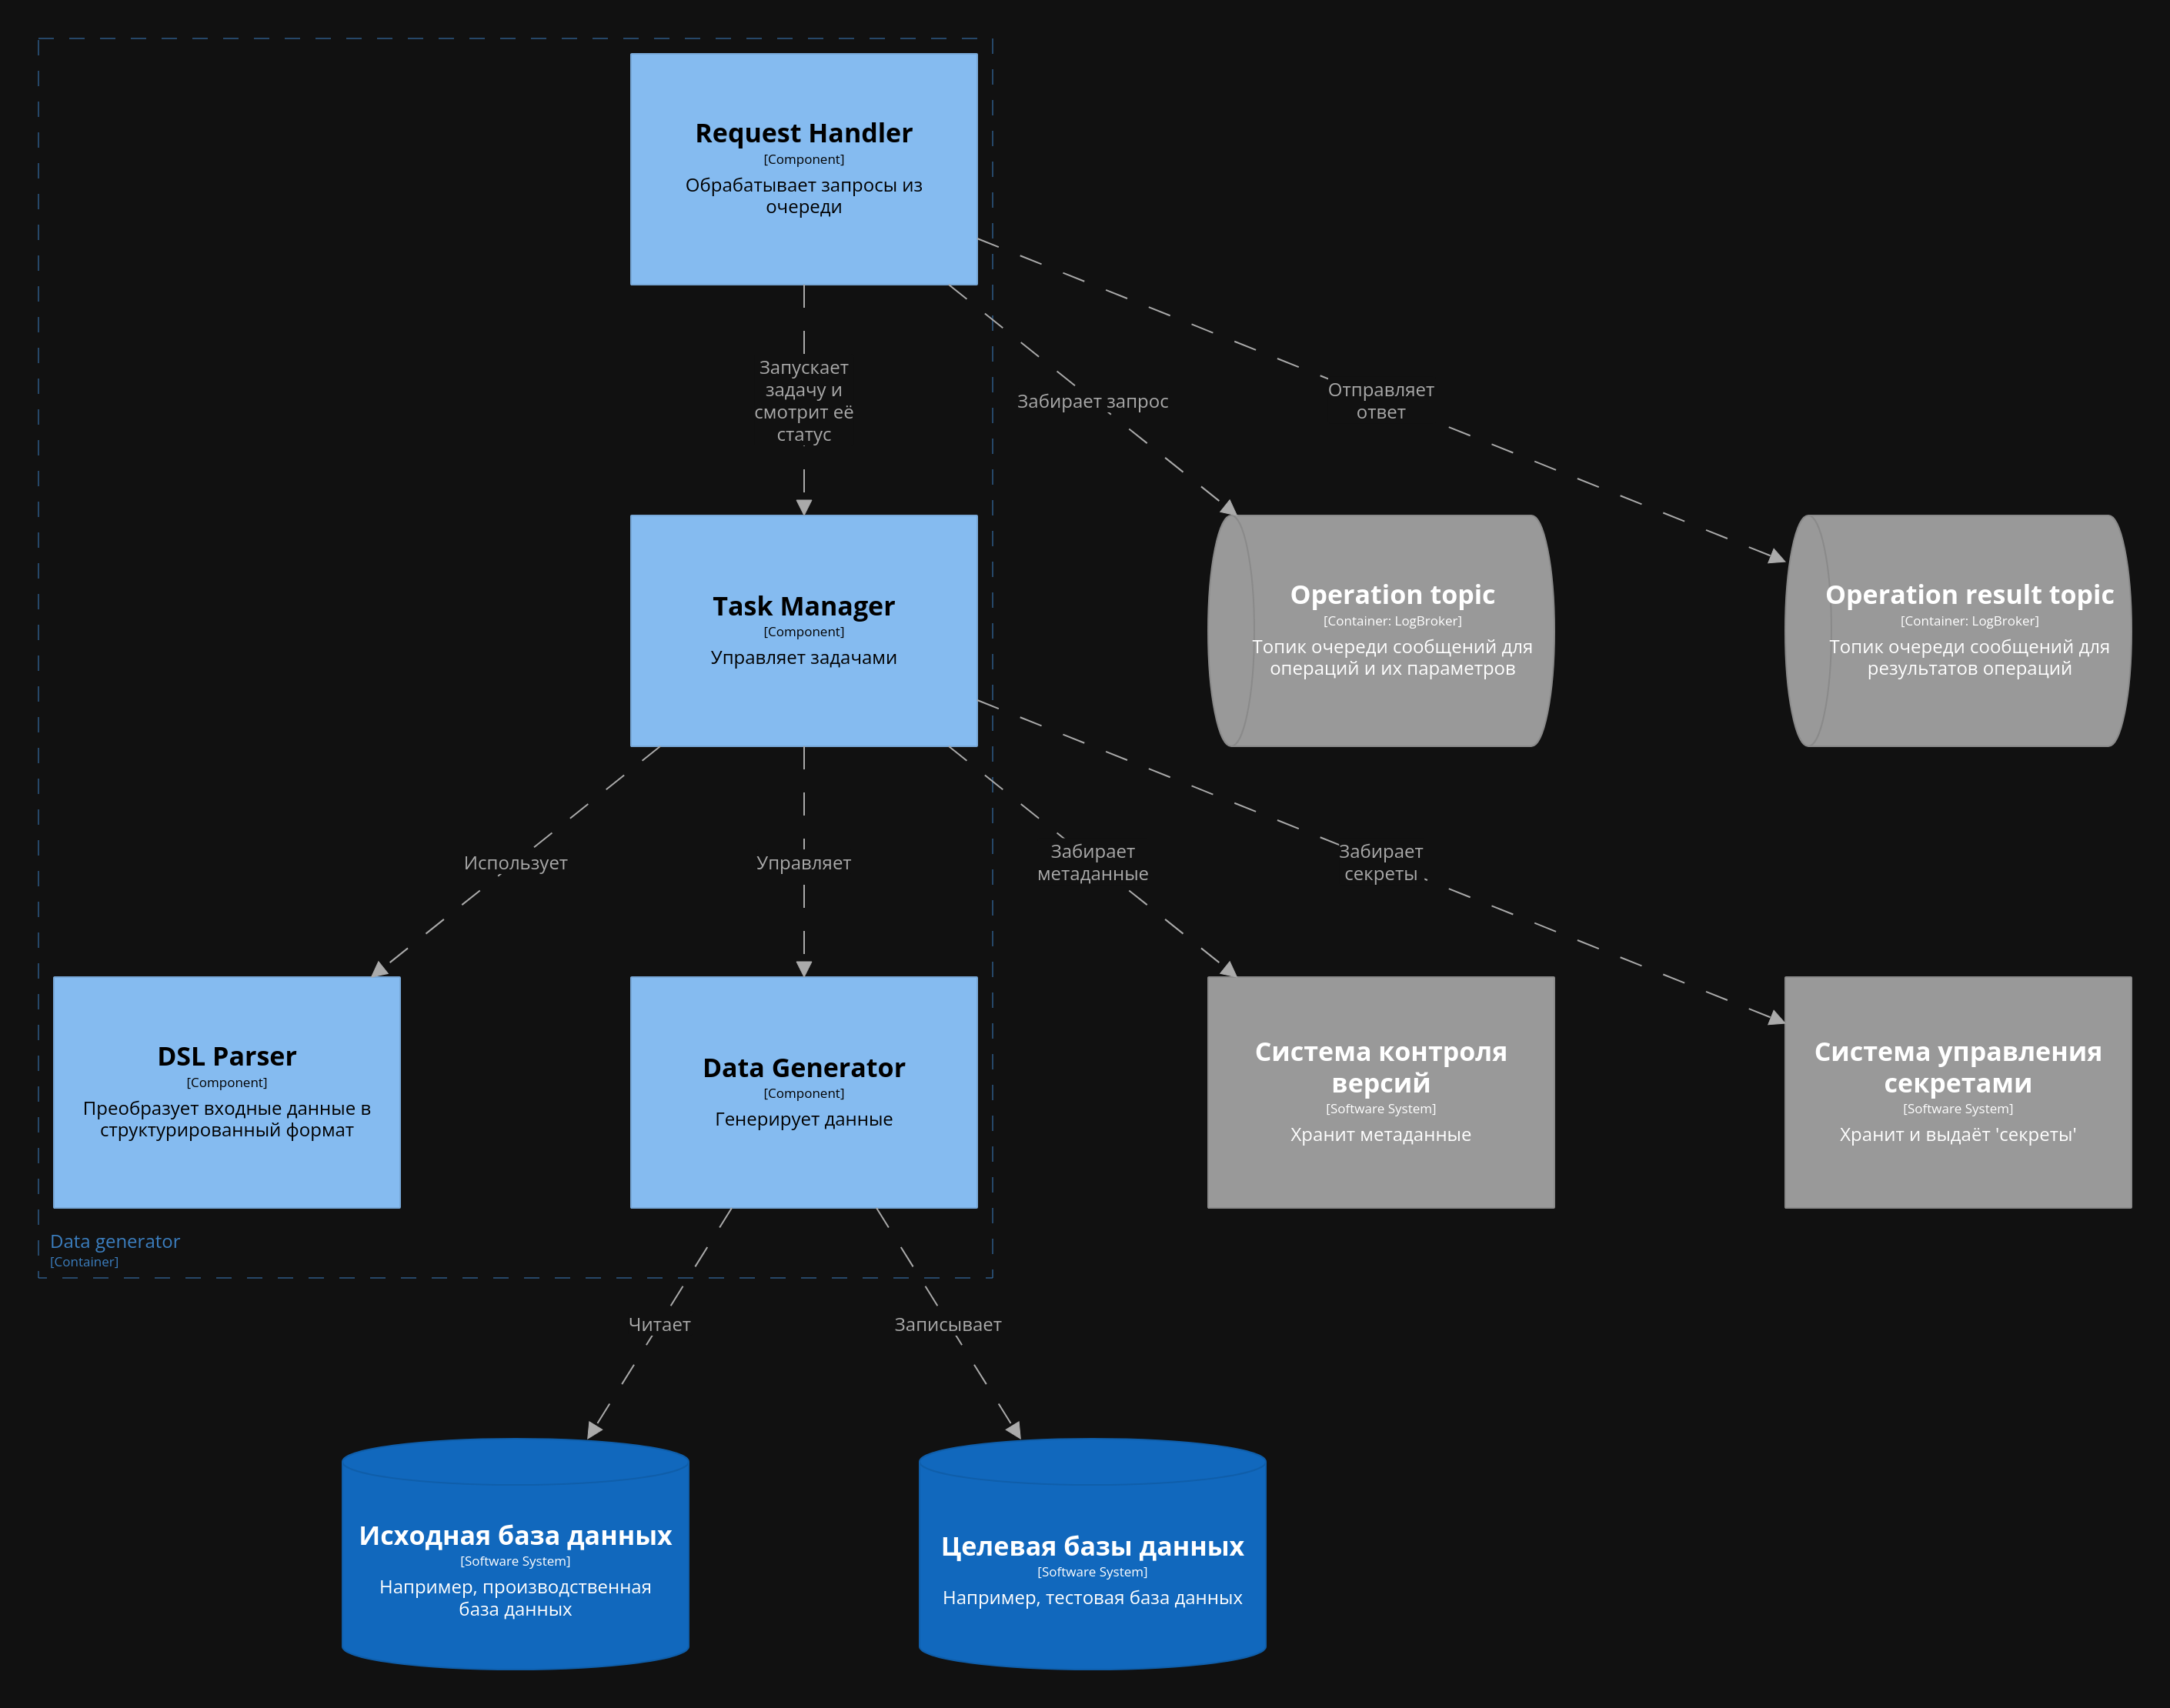
\includegraphics[scale=0.15]{./img/structurizr-DataGeneratorComponents.png}
  \caption{Data Generator Components}
  \label{data-generator-components}
\end{figure}

\subsection{Метаграфы}
TBD: расписать эту секцию получше

$MG = <V, MV, E, ME> $ -- метаграф, где $V$ -- множество вершин, $MV$ -- множество метавершин, $E$ -- множество рёбер, $ME$ -- множество метарёбер.

$v_i = \{atr_k\}, v_i \in V$, где $v_i$ -- вершина, $atr_k$ -- атрибут.

$mv_i = <\{v_j\}, \{atr_k\}>, mv_i \in MV, v_j \in V$, где $mv_i$ -- метавершина, $v_j$ -- вершина, $atr_k$ -- атрибут.

$e_i = <v_s, v_e>, e_i \in E, v_s, v_e \in V$, где $e_i$ -- ребро, $v_s$ -- исходная вершина, $v_e$ -- конечная вершина.

$me_i = <mv_s, mv_e, \{atr_k\}>, me_i \in ME, mv_s, mv_e \in MV$, где $me_i$ -- метаребро, $mv_s$ -- исходная метавершина, $mv_e$ -- конечная метавершина, $atr_k$ -- атрибут.

Ограничение: $\forall mv_i, mv_j \in V, i \neq j => \{v_x\}_i \cap \{v_y\}_j = \emptyset$

\subsection{Алгоритм переноса данных}
TBD: расписать эту секцию получше

Для реляционной базы данных метаграф это:
\begin{itemize}
  \item вершины обозначают данные; атрибуты -- полезная нагрузка;
  \item метавершины обозначают таблицы, содержащие данные; атрибуты -- структура таблицы;
  \item рёбра показывают, как связаны данные;
  \item метарёбра показывают, как связаны таблицы (по Foreign Key); атрибуты -- названия полей, по которым связаны таблицы.
\end{itemize}

\begin{figure}
  \fontsize{12pt}{14pt}\selectfont
  \begin{lstlisting}
// TBD: написать алгоритм
BFSforMetagraph(graph, startVertex)
   // Инициализация
   queue := {}
   visited := {}
  \end{lstlisting}
  \caption{Алгоритм }
\end{figure}
